\documentclass[12pt]{article}
\usepackage[margin=1in]{geometry}
\geometry{letterpaper}
\usepackage{doc}
\usepackage{url}
\usepackage{lastpage}
\usepackage{graphicx}
\usepackage{gensymb}
\usepackage[section]{placeins}
\usepackage{fancyhdr}
\usepackage{tikz}
\usetikzlibrary{shapes,arrows}
\tikzstyle{block} = [rectangle, draw, fill=blue!20, 
     text centered, rounded corners, minimum height=2em]
\tikzstyle{line} = [draw, -latex']
\usepackage{hyperref}
\usepackage[belowskip=-50pt,aboveskip=2pt]{caption}
% \setlength{\intextsep}{8pt plus 2pt minus 2pt}

\title{IARC Technical Paper}
\author{
	\textbf{Texas Aerial Robotics} \\ 
	\textit{University of Texas at Austin} \\ \\ 
%	Austin, TX 78705 \\ 
	\href{mailto:TexasAerialRobotics@gmail.com}{TexasAerialRobotics@gmail.com} \\ \\ 
	Samid Ahmed, Nicholas Boeker, Eric Johnson, \\ Aaron Karns, Mark Loveland, Umer Salman} 

\date{May 28, 2017}

\pagestyle{fancy}
\renewcommand{\headrulewidth}{0pt}
\fancyhead{}
\cfoot{\textsf{Page \thepage\ of \pageref{LastPage}}}

\begin{document}
\maketitle
\thispagestyle{empty}

\abstract{
Texas Aerial Robotics will compete in Mission 7 of the International Aerial Robotics Competition (IARC) in 2017. Our goal is to direct Roombas (iRobot Create 2's), known as ground robots, using a quadcopter equipped with a camera (put name here) for vision, a Nvidia Jetson for vision processing, and a Pixhawk for controlling the quadcopter. The mission takes place in a GPS denied environment, so gridlines will be used as reference positions. 
}

\pagebreak
\tableofcontents

\pagebreak

\section{Introduction}
\subsection{The Mission}
Mission 7a of IARC consists of developing an aerial vehicle that can interact with moving ground robots. Those ground robots, or Roombas, have randomized movements so the aerial vehicle must make decisions on the fly rather than having preprogrammed instructions. The vehicle must herd the 10 Roombas across one side of the 20 meter by 20 meter grid. Additionally, 4 obstacle Roombas have PVC poles the vehicle must avoid. The way the vehicle must herd the Roombas is by either blocking the forward motion of the Roomba, directing it to rotate 180\degree, or tapping the pressure plate atop the Roomba, directing the Roomba to rotate 45\degree clockwise. 

An added difficulty to the mission is that the setting is a (Global Positioning System) GPS denied environment. Additionally, there are no landmark features to allow the vehicle to use Simultaneous Localization and Mapping (SLAM) for orientating itself on the grid. Thus, we determined that we needed to design other methods to determine our positioning. By using a camera to observe the gridlines and an Inertial Measurement Unit (IMU), we are working our way to determining where the vehicle is on the grid. 

Mission 7b will add in an additional aerial vehicle to compete against for herding more Roombas. 

\subsection{Yearly milestones}
This is the first time Texas Aerial Robotics is competing in any event. Our goal for the year was to be competitive at this year's IARC. 

\subsection{Faculty Support}
At the beginning of the creation of Texas Aerial Robotics, the team searched for professors to provide technical guidance for the project. Within the UT Department of Aerospace TAR reached out to Dr. Maruthi Akella. Dr. Akella has been conducting research in areas similar to the core objectives of IARC’s Mission 7. Dr. Akella has been doing research to create agile intelligent quadrotors in environments free of GPS. Dr. Akella expressed interest in Mission 7 as soon the team reached out. From the outset of the relationship Dr. Akella has provided expertise, access to his grad students as well as access to his indoor and outdoor lab. Dr. Akella also introduced us to multiple corporation looking to sponsor student projects. TAR is incredibly thankful to have the support of Dr. Akella. 

\subsection{Team Structure}
As important as the drone a team develops, is the process in which it is developed. The past year has been Texas Aerial Robotics(TAR) maiden year and the team has put a lot of effort in developing the process to catalyze the engineering of the drone. During the fall semester, the team made just about every mistake in the book with regards to how to run a competition team. The team struggled with communication, vision and drive. This disorganization resulted with TAR ending the first semester with little to no progress. With the failure of the semester came the resignation of our president. Texas Aerial Robotics was at a crossroads. 

The winter break was used as a period of reflection. At the start of the new semester a new president was elected and a formal management style was implemented: Scrum. This is short term, agile style of management that makes short term goals and reflects and resets for the next “scrum”. Along with scrum, the team implemented organizational apps such as Slack and Trello. Slack allowed the team to keep all the sub-team conversations separate, but unified. This kept members from silencing their line of communication as well as still allowing members to view what the other sub-teams are working on. Automated reminders for meetings were also set up through Slack to prevent members from forgetting their duties to the team. Trello was an incredible addition to our organizational platform. Trello is a ubiquitous bulletin board in which we can make and assign tasks throughout the team. This has helped to promote accountability as well as allow the better delegation of jobs. Finally, the last big productivity mechanism we implemented was the formation of a business/logistics subteam. This team has allowed the engineers to focus on engineering by acquiring money and organizing logistics, such as the trip to Atlanta. 

\subsection{Budget}
The UT Aerospace Department was the first institution to support the team. TAR received a couple thousand dollars to begin our project as well as permission to use the aerospace facilities. After doing cost analysis TAR set the target budget at \$10,000. The team’s big break came after reaching out to Dr. Maruthi Akella. As well as providing the team with technical guidance, Dr. Akella introduced us to executives from corporations looking to sponsor student projects. Of the two corporations TAR reached out to, General Dynamics Mission Systems (GDMS) decided to fully sponsor us at the requested budget. The team is extremely grateful to have received the support of GDMS. Without this relationship, the development and trip to Atlanta would not have been possible. 

\section{Quadcopter}

After our initial brainstorming period the team decided that the drone would would need to be able to easily interact with Roombas, fly at least 10 min and have a large body to accommodate for the many electronics. At the beginning of our design process the team was faced with the prospects of buying, or designing and building a drone in house. After doing research, the design team decided that no prebuilt could fully meet the needs. The team decided to use the propeller guards as a forward blocking surface as well as a safety feature. To get the propeller guards to the required height to block the Roombas the team chose to have the body of the drone be the landing gear. Surface area of the drone was elected to be maximized to decrease the precision needed to contact the top of the Roombas. The quadcopter would be made with aluminum arms with a carbon fiber base to minimize weight and maximize strength and build quality. During build, we laser-cut wood for the base to allow for rapid iterating. Rapid iteration was instrumental in finding the optimal layout of electronics as well as flush out design flaws. Using wood also meant that we would be dealing with more magnetic interference and vibration than we would after switching to carbon fiber, allowing us to test with worse conditions. The body of the drone was designed from the outset to keep the electronics easily accessible. For this reason a removable base cover was implemented. 

We decided to fabricate a quadcopter with aluminum arms with a carbon fiber base. During build, we laser-cut wood for the base to allow for rapid iterating. Using wood also meant that we would be dealing with more magnetic interference and vibration than we would after switching to carbon fiber, allowing us to test with worse conditions. Our quadrotor needed to house all of the sensors for operation with sufficient flight time. 

\begin{figure}[!htbp]
\begin{center}
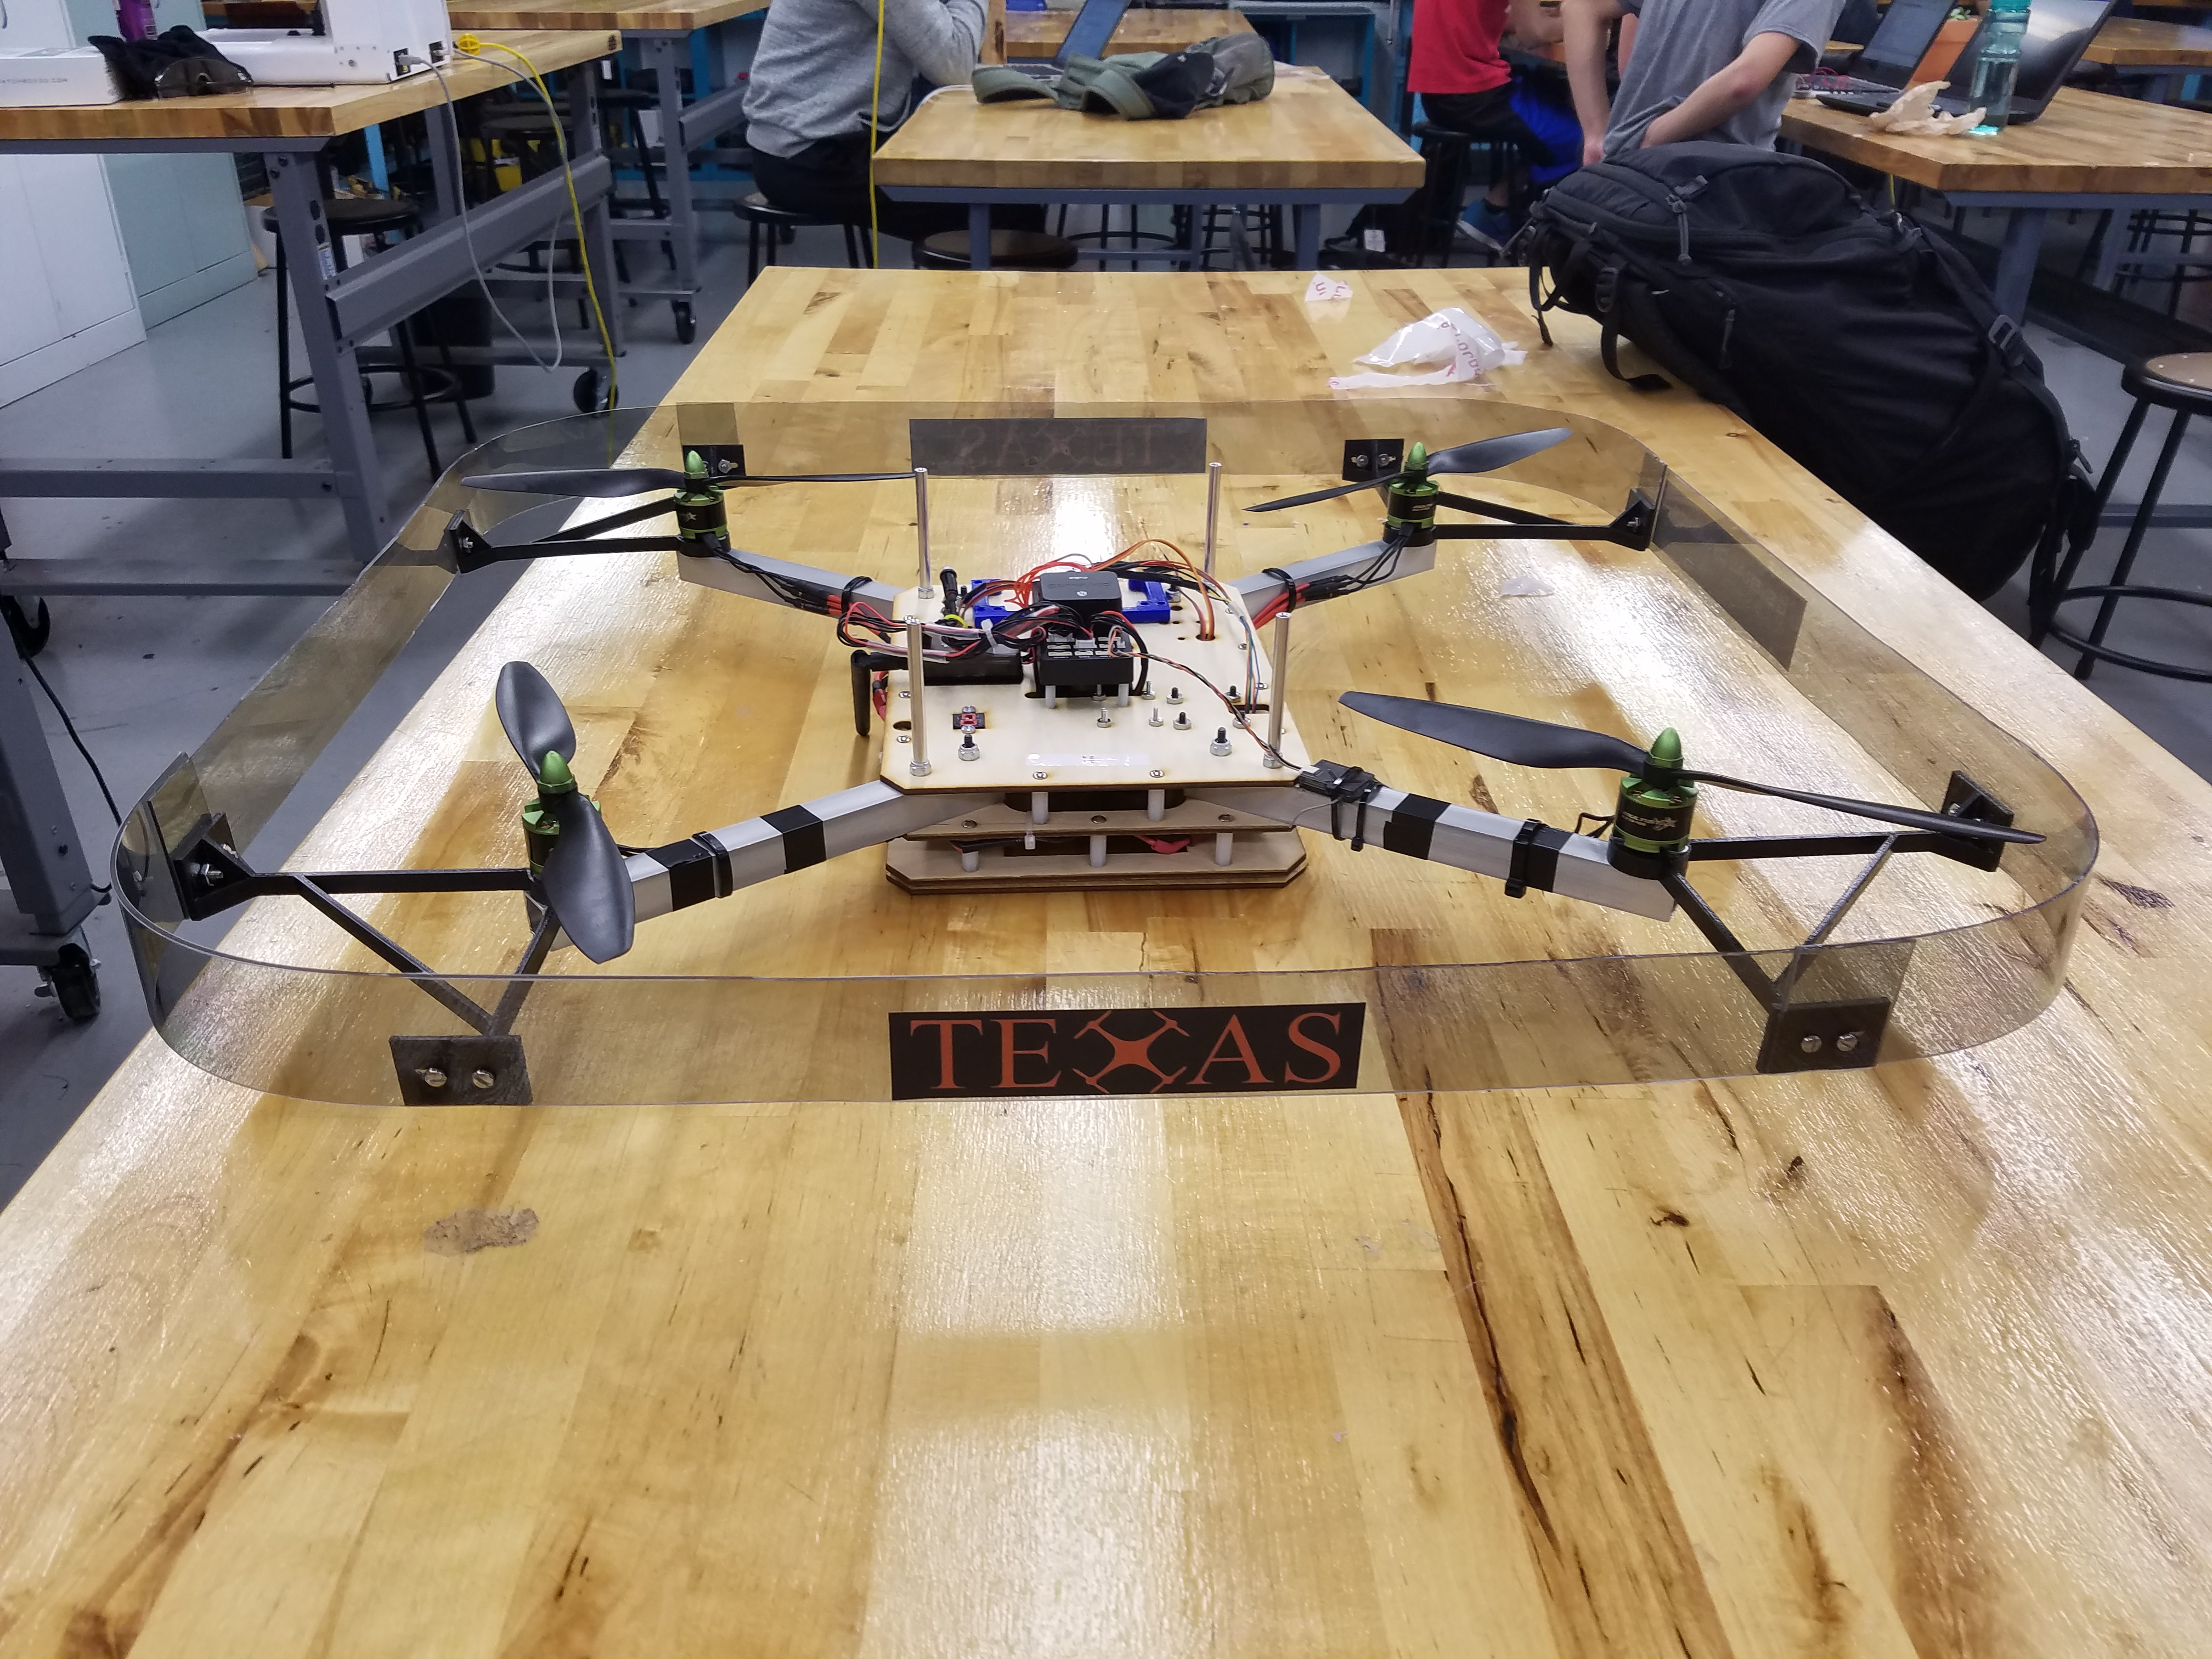
\includegraphics[width=0.75\textwidth]{quad}
\caption*{Quadcopter during testing phase}
\end{center}
\end{figure}

\subsection{Hardware} 
At the end of the aluminum arms sit four (insert here) motors for lift. The four motors provide (insert) grams of lift, a sufficient amount for our (insert) gram quadcopter. The arms are fixed into the base pieces, which do not pass enough vibration to the sensors that we needed any additional vibration damping. 

\begin{figure}[!htbp]
\begin{center}
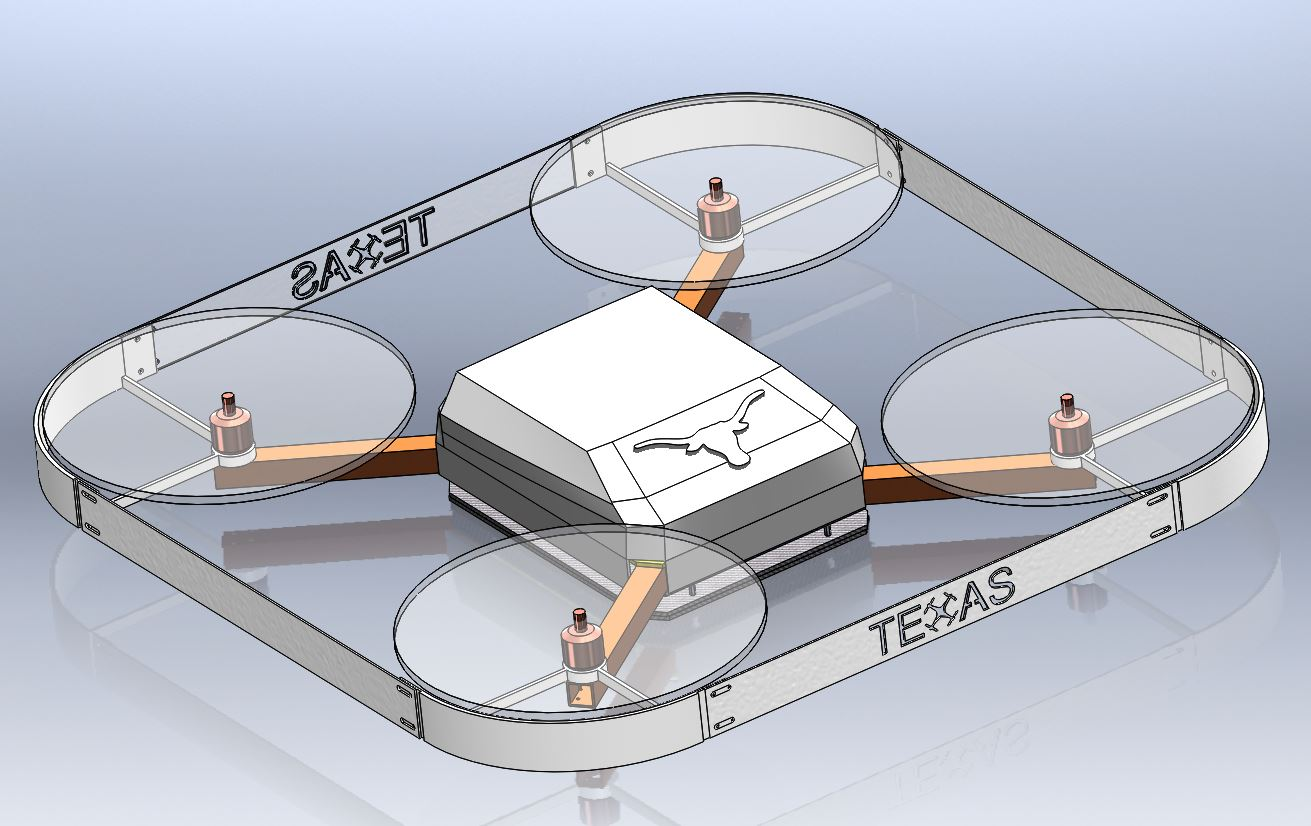
\includegraphics[width=0.75\textwidth]{render}
\caption*{SOLIDWORKS render of quadcopter}
\end{center}
\end{figure}
\subsection{Controls}
We use a Pixhawk flight controller, situated directly center of the quadcopter, for flying and sensor capabilities. We supplement the Pixhawk's accelerometer, gyroscope, and compass with an optical flow sensor (PX4FLOW) for position tracking and a LIDAR (LIDAR Lite v3) for altitude measurements. These sensors allow the Pixhawk to better maneuver and stabilize the flight of the vehicle. 

Both the optical flow sensor and the LIDAR sensor integrate with the Arducopter flight software that is running on the Pixhawk. The optical flow sensor is mounted on the side of the main body of the quadcopter to ensure that sensor receives adequate lighting at all times. 
\begin{figure}[!htbp]
\begin{center}
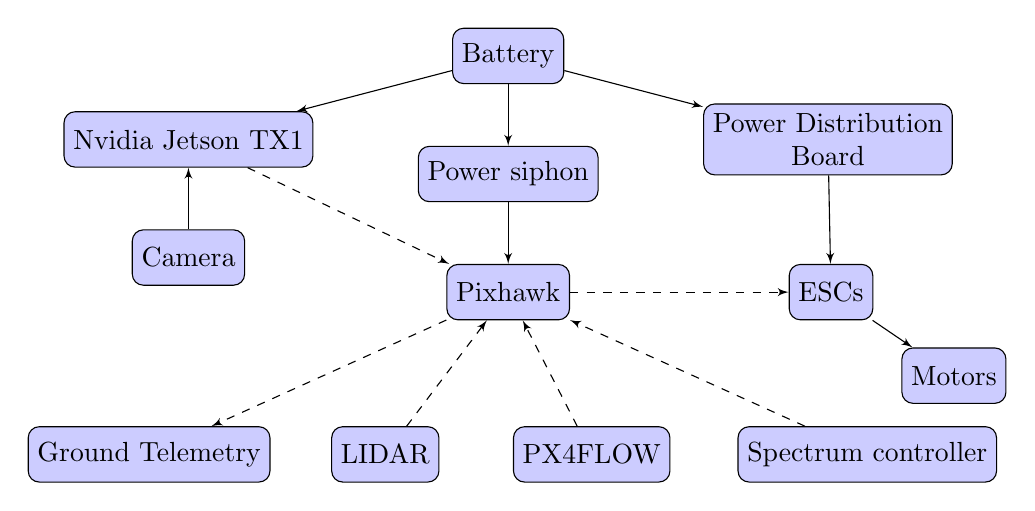
\begin{tikzpicture}[node distance = 1.5cm and 8cm, auto]
    % Place nodes
    \node [block] (battery) {Battery};
    \node [block, below of=battery] (siphon) {Power siphon};
    \node [block, below of=siphon] (Pixhawk) {Pixhawk};
    \node [block, below right of=battery, xshift=3cm, align=center] (PDB) {Power Distribution \\ Board};
    \node [block, below left of=battery, xshift=-3cm] (Jetson) {Nvidia Jetson TX1};
    \node [block, right of=Pixhawk, xshift=2.6cm] (ESCs) {ESCs};
    \node [block, below right of=ESCs, xshift=.5cm] (Motors) {Motors};
    \node [block, below of=Jetson] (Camera) {Camera};
    \node [block, below right of=Pixhawk, yshift=-1cm] (Flow) {PX4FLOW};
    \node [block, below right of=Pixhawk, xshift=3.5cm, yshift=-1cm] (Spectrum) {Spectrum controller};
    \node [block, below left of=Pixhawk, xshift=-.5cm, yshift=-1cm] (LIDAR) {LIDAR};
    \node [block, below left of=Pixhawk, xshift=-3.5cm, yshift=-1cm] (Telemetry) {Ground Telemetry};
    % Draw edges
    \path [line] (battery) -- (siphon);
    \path [line] (siphon) -- (Pixhawk);
    \path [line] (battery) -- (PDB);
    \path [line] (PDB) -- (ESCs);
    \path [line] (battery) -- (Jetson);
    \path [line] (Camera) -- (Jetson);
    \path [line, dashed] (Flow) -- (Pixhawk);
    \path [line, dashed] (Jetson) -- (Pixhawk);
    \path [line, dashed] (LIDAR) -- (Pixhawk);
    \path [line, dashed] (Pixhawk) -- (Telemetry);
    \path [line, dashed] (Spectrum) -- (Pixhawk);
    \path [line, dashed] (Pixhawk) -- (ESCs);
    \path [line] (ESCs) -- (Motors);
\end{tikzpicture}
\caption*{Solid arrows indicate power while dashed lines indicate power+data}
\end{center}
\end{figure}
\subsection{Vision}

The drone tracks the Roombas as well as keeps its global position using data taken from the camera mounted facing downwards. The Jetson TX1 is what the drone uses to take the data from the camera and run our custom computer vision programs. We use the free OpenCV libraries to assist in our computer vision algorithms. 

In order to track the Roombas, we opted to exploit the fact that the tops of the Roombas are taped in either a distinct shade of red or green. This is done by applying a simple threshold and localizing the region in which the colored pixels are detected. With height input from the LIDAR, the computer vision algorithm can easily convert distance in pixels to distance in meters. This allows us to know the distances of the Roombas relative to the drone. From here we can combine this data with our grid tracking algorithm and computational model to map the Roombas globally.

The algorithm for keeping the drone’s position within the grid relies on line detection. This is achieved by applying many operations to a standard RGB image. First, the image passes through the camera as an RGB picture. The image is then converted to grayscale. Next, the Canny Edge detection [1] filters the grayscale image into a binary image. From there, the binary image is fed through a Hough Transform [2] that essentially takes the binary image and outputs vectors which end up being the grid lines. The algorithm then reads these vectors and sorts them into two bins based off of the direction that they point [3]. Once sorted, the closest vector in each group to the center of the image is found. The distance can be used to calculate distance within each grid square. Each time the center of the drone’s camera passes over a line, the grid square number is also updated.

Below is a flowchart to illustrate our tracking algorithms: \\ \\ 
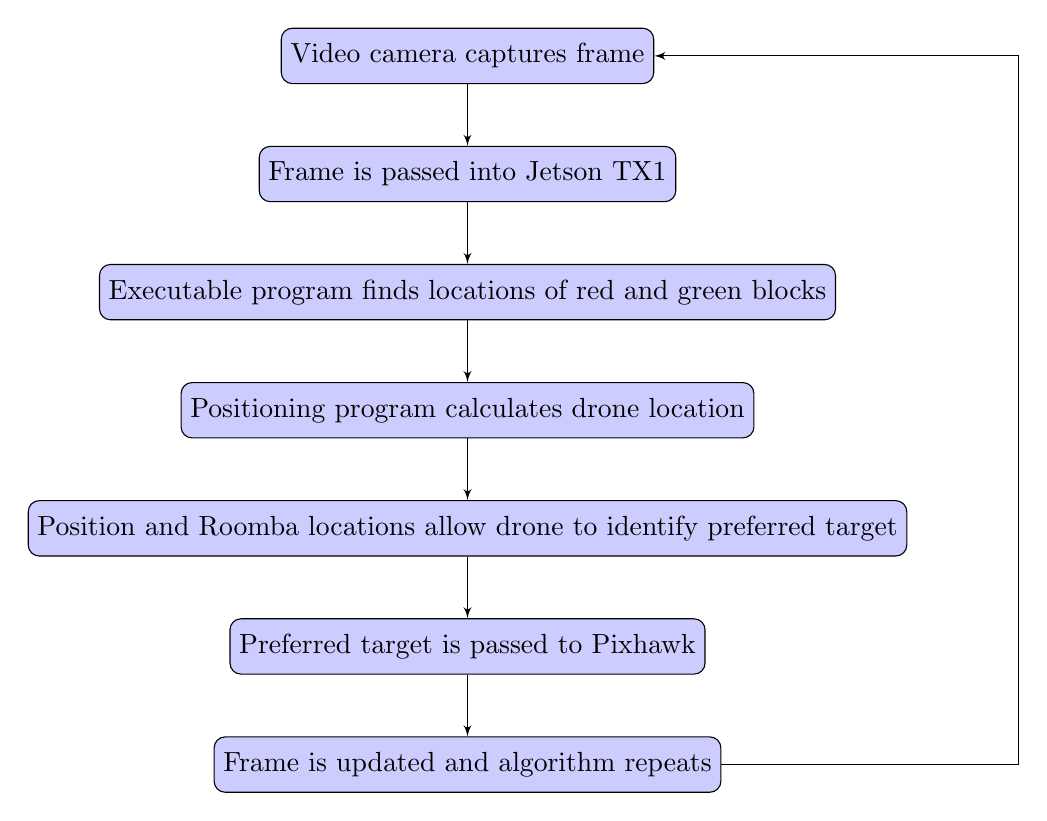
\begin{tikzpicture}[node distance = 1.5cm, auto]
    % Place nodes
    \node [block] (camera) {Video camera captures frame};
    \node [block, below of=camera] (passed) {Frame is passed into Jetson TX1};
    \node [block, below of=passed] (find) {Executable program finds locations of red and green blocks};
    \node [block, below of=find] (calc) {Positioning program calculates drone location};
    \node [block, below of=calc] (preferred) {Position and Roomba locations allow drone to identify preferred target};
    \node [block, below of=preferred] (passpreferred) {Preferred target is passed to Pixhawk};
    \node [block, below of=passpreferred] (update) {Frame is updated and algorithm repeats};
    % Draw edges
    \path [line] (camera) -- (passed);
    \path [line] (passed) -- (find);
    \path [line] (find) -- (calc);
    \path [line] (calc) -- (preferred);
    \path [line] (preferred) -- (passpreferred);
    \path [line] (passpreferred) -- (update);
    \path [line] (update) -- ++(7cm,0) |- (camera);
\end{tikzpicture}

\begin{center}
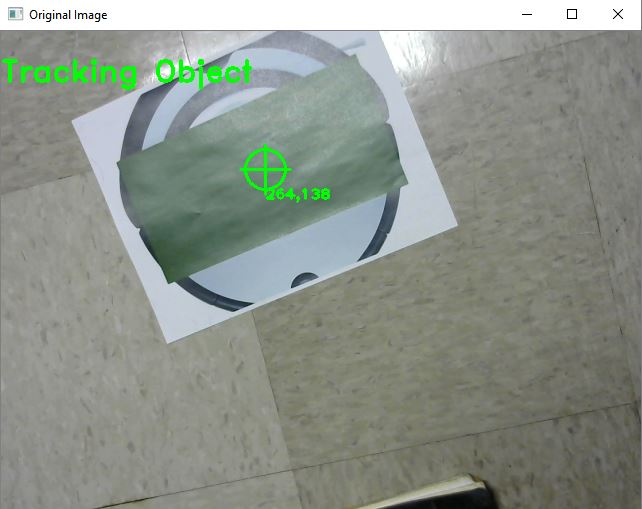
\includegraphics[width=0.8\textwidth]{tracking}
\end{center}

\section{Safety}
\subsection{Preflight Checklist}
\begin{enumerate}
	\item Check LIDAR and flow sensor are not covered 
	\item Check ESCs are plugged into correct ports 
	\item Check props are on in the correct direction 
	\item Check props are not upside down
	\item Check that drone is level before powering on
	\item Hold safety button
	\item Make sure ground station has good telemetry
	\item Verify critical sensors are giving good data
	\item Make sure everyone is clear of drone 
\end{enumerate}

\subsection{Kill Switch}
Hopefully we will have a Kill Switch 

\subsection{Prop Guards}
Our prop guards took multiple iterations. We wanted a design that would not interfere with the prop wash, but still be able to avoid the quadcopter from destroying itself in the unfortunate event it collides with something. The first iteration looked nice, but interfered with the prop wash too much and weighted too much, reducing the thrust. 

\section{Simulations}
Another aspect of our research into solving Mission 7 involved simulating the arena and quadcopter on the computer to allow us to test without fear of damaging the quadcopter. It also allowed us to test with a full field and simulated Roombas as we currently do not have a physical field setup or more than one Roomba. 

\begin{center}
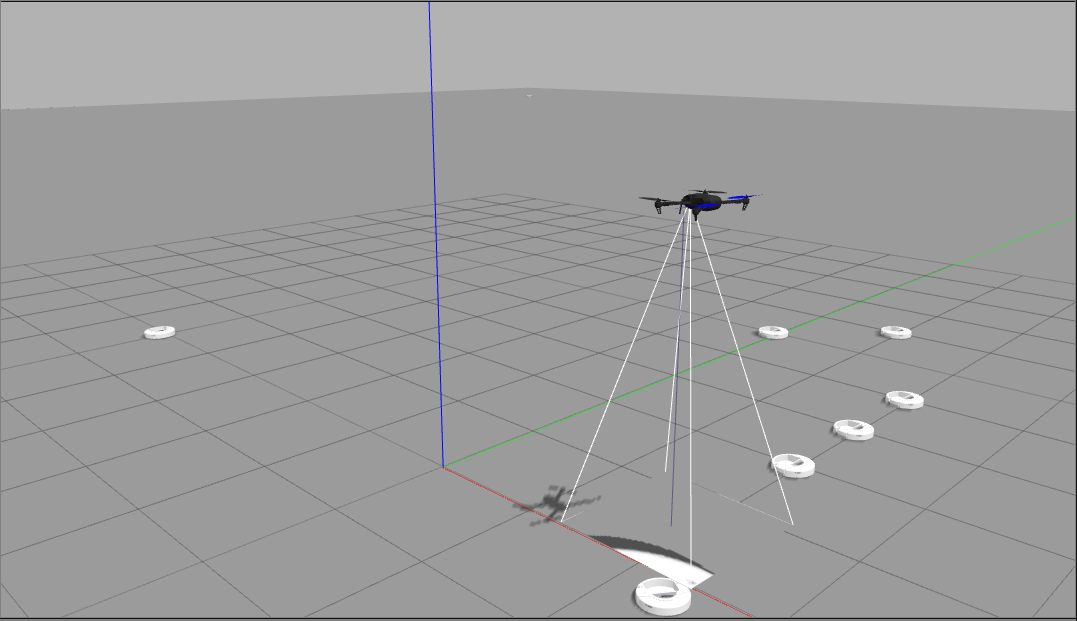
\includegraphics[width=0.8\textwidth]{Selection_004}
\end{center}

To simulate the quadcopter, we use Ardupilot's Software in the Loop (SITL) simulation method to run a Gazebo simulation with ROS. Using the PX4 flight stack, we are able to simulate a quadcopter like ours with a Pixhawk and Optical Flow sensor. 

To simulate the Roombas, we use a SDF model found online which we duplicated to get the 10 objective Roombas and 4 obstacle Roombas. We can simulate the randomized motion by issuing ROS commands to the Roombas. 

\section{Conclusion}
We still have quite a ways to go before we can consider ourselves competitive. Due to the fact that we started our organization in 2017, we have come a long way and learned a lot, yet we plan to continue work to beat this mission as quick as possible. Hopefully we do well at Georgia Tech! 

\section{Acknowledgments}
We are thankful for Dr. Akella at UT Austin. Additionally, we are thankful for UT Austin's Aerospace Department for providing us with a meeting room and sponsorship. 

We also would not have been able to work towards this mission without the sponsorship of General Dynamics. 
\bibliography{Paper}
\bibliographystyle{unsrt} 

\end{document}
